\documentclass[a4paper]{article}
\usepackage[T1]{fontenc}
\usepackage{listings}
\lstset{
 basicstyle=\ttfamily
}
\usepackage{verbatim}
\usepackage[utf8]{inputenc}
\usepackage[italian]{babel}
\usepackage{lipsum}
\usepackage{graphicx}
\author{Anis Lico \and Simone Del Gatto}
\title{Programmazione di reti - Relazione Assigment 2}
\begin{document}
\maketitle

\tableofcontents

\section{Descrizione Simulatore}
Il simulatore si articola principalmente in due parti il lato sender rappresentato dall'entità A  e il lato reciver rappresentato da B.
Con \emph{A\_init()} e \emph{B\_init()}, chiamate subito all'inizio dell'esecuzione, vengono inizializzate variabili e strutture dati relative alle due entità.
All'inizio del programma viene creata una struttura dati che indica quali eventi si devono verificare durante l'esecuzione e in che ordine. Tramite apposite funzioni, come ad esempio \emph{tolayer3()} o \emph{starttimer()}, si possono aggiungere eventi a questa lista. 
Il main si preoccuperà di simulare la la ricezione di un messaggio da parte di A proveniente dal layer 5 e di far si che A lo invii tramite la funzione \emph{A\_output()}. A utilizzando la funzione \emph{tolayer3()} si preoccuperà di inviare il messaggio a B. Dal punto di vista della simulazione questo significa che viene aggiunta alla lista degli eventi un evento che sarà del tipo "B riceve un pacchetto da A". Quando effettivamente questo evento si realizzerà il simulatore chiamerà la funzione \emph{B\_input()} che nel caso il pacchetto ricevuto sia quello corretto spedirà un ack all'entità A tramite la funzione \emph{tolayer3()} e spedirà il pacchetto al livello applicativo soprastante tramite la funzione \emph{tolayer5()}. Quando si attuerà l'evento che determina la ricezione da parte di A di un ack inviatogli da B, se il pacchetto è quello previsto A si prepara a inviare nuovi pacchetti provenienti dal livello 5 (una spiegazione più dettagliata dell'implementazione delle routine è fornità successivamente).
Il simulatore mette a disposizione anche un timer che viene controllato tramite le due funzioni \emph{starttimer()} e \emph{stoptimer()}. A utilizzare questo timer sarà unicamente A che lo avvierà al momento dell'invio di un pacchetto e lo farà terminare al momento della corretta ricezione di un ack (la gestione del timer sarà rivista poi in maniera più approfondita successivamente). Allo scadere del timer, dovuta alla non corretta ricezione dell'ack o perché quest'ultimo non è proprio arrivato o per un fenomeno di corruzione dei pacchetti, il simulatore chiama la funzione \emph{A\_timerinterrupt()} che permette il riinvio del pacchetto attualmente non ackato.
\begin{figure}[h!]
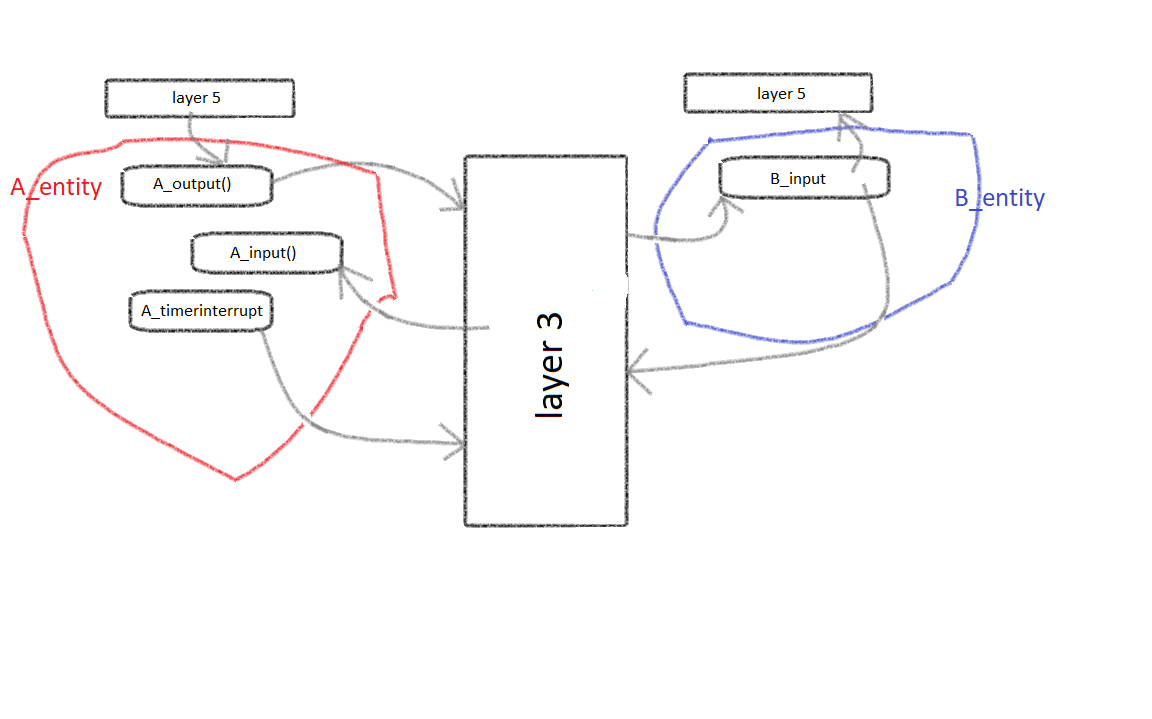
\includegraphics[scale = 0.60]{Immagine.png}
\caption{Schema simulatore}
\end{figure}
\section{Strategie Risolutive}

\subsection{Strutture Dati}
\begin{itemize}
\item \textbf{messToSend}: è una struttura che di permette di realizzare una coda per 			bufferizzare i messaggi che devono essere inviati da A a B. 

\item \textbf{messagesList}: puntatore alla testa della coda che indica il prossimo 			messaggio da inviare. Questo è necessario perché il simulatore potrebbe far si che il livello 5 cerchi di far inviare un messaggio tramite A mentre questo è in fase di attesa di un ack da B. Non potendolo inviare in quel momento lo può bufferizzare per poi inviarlo successivamente.

\item \textbf{currentPacket}: puntatore al pacchetto in inviato da A che deve essere ackato. Questa struttura dati si rende necessaria per avere un riferimento attraverso la quale si può ritrasmettere eventualmente il pacchetto.
\end{itemize}

\subsection{Descrizione delle Routine}
\begin{itemize}

\item \textbf{A\_init}: inizializza le strutture e le variabili relative ad A.

\item \textbf{B\_init}: inizializza le strutture e le variabili relative ad B
.
\item \textbf{A\_output(message)}: si controlla la variabile \emph{state} che può avere due valori: \emph{CAN\_SEND\_MESSAGE} che indica che si può procedere con l'invio di un messaggio e \emph{WAITING\_ACK} che indica che si è in attesa di un acknolegment da B. E' chiaro che se B ha come valore \emph{CAN\_SEND\_MESSAGE} si può procedere con l'invio e l'avvio del timer tramite \emph{starttimer()}, in caso contrario il messaggio sarà bufferizzato in \emph{messagesList}. 

\item \textbf{A\_input(packet)}: si possono verificare due situazioni
\begin{enumerate}
\item il pacchetto ricevuto non è corrotto e ha il numero di acknolegment uguale a quello atteso da A: viene stoppato il timer e si guarda se nella lista dei messaggi ci sono dei messaggi bufferizzati. In caso affermativo viene inviato il primo della coda e la variabile state viene settata a \emph{WAITING\_ACK}. In caso contrario a si prepara a inviare nuovi messaggi provenienti dal livello 5 settando la variabile state a \emph{CAN\_SEND\_MESSAGE}

\item il pacchetto è corrotto o ha un numero di ack non atteso: viene riinviato il messaggio puntato da \emph{currentPacket}.

\end{enumerate} 

\item \textbf{A\_timerinterrupt()}: viene ritrasmesso il pacchetto puntato da \emph{currentPacket}

\item \textbf{B\_input(packet)}: possono verificarsi due casi:
\begin{enumerate}
\item il pacchetto ricevuto è corretto e il suo sequence number è quello atteso da B. Viene inviato un ack con acknum uguale a seqnum del pacchetto e il pacchetto viene consegnato al livello 5 tramite la funzione \emph{tolayer5()}. 
\item il pacchetto ricevuto o è corrotto o ha un sequence number non atteso (magari frutto di una ritrasmissione). Viene inviato un ack con acknum uguale all'opposto numero di sequenza che B si aspettava di trovare nel pacchetto ricevuto da A
\end{enumerate}

\end{itemize}

\subsection{Diagrammi a stati finiti}
Macchine a stati finiti per la descrizione del comportamento dell'entità A e dell'entità B
\begin{figure}[h!]
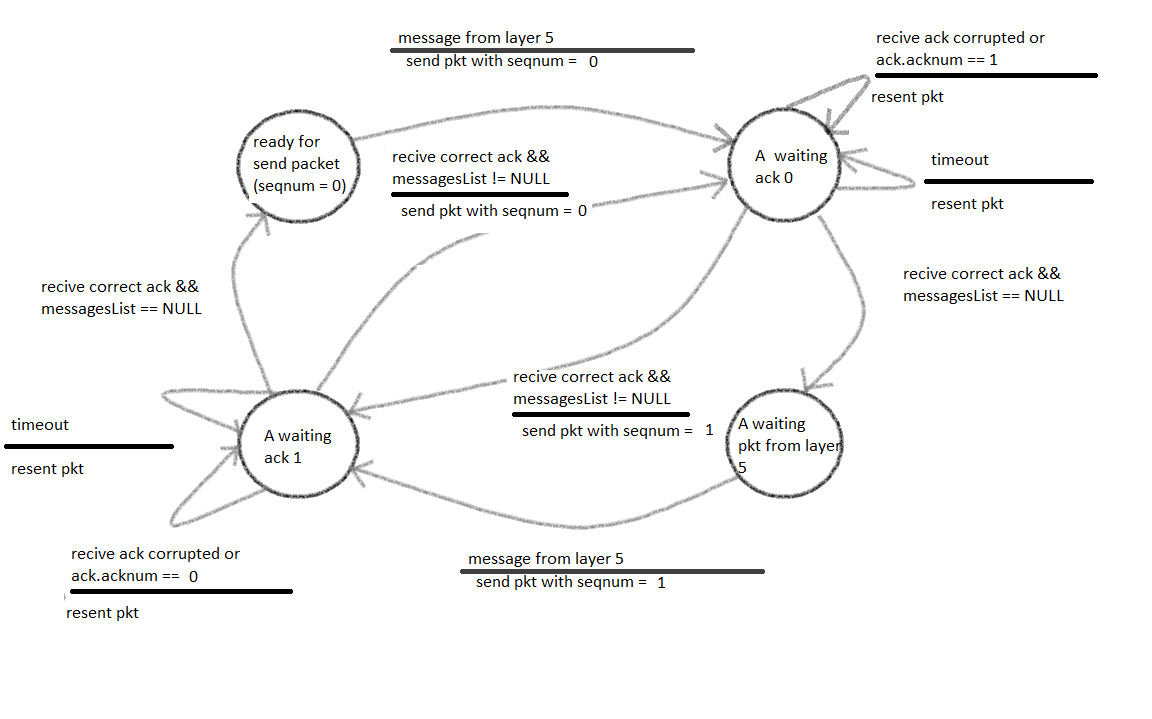
\includegraphics[scale = 0.40]{A.png}
\caption{Diagramma a stati entità A}
\end{figure}
\newline
\begin{figure}[h!]
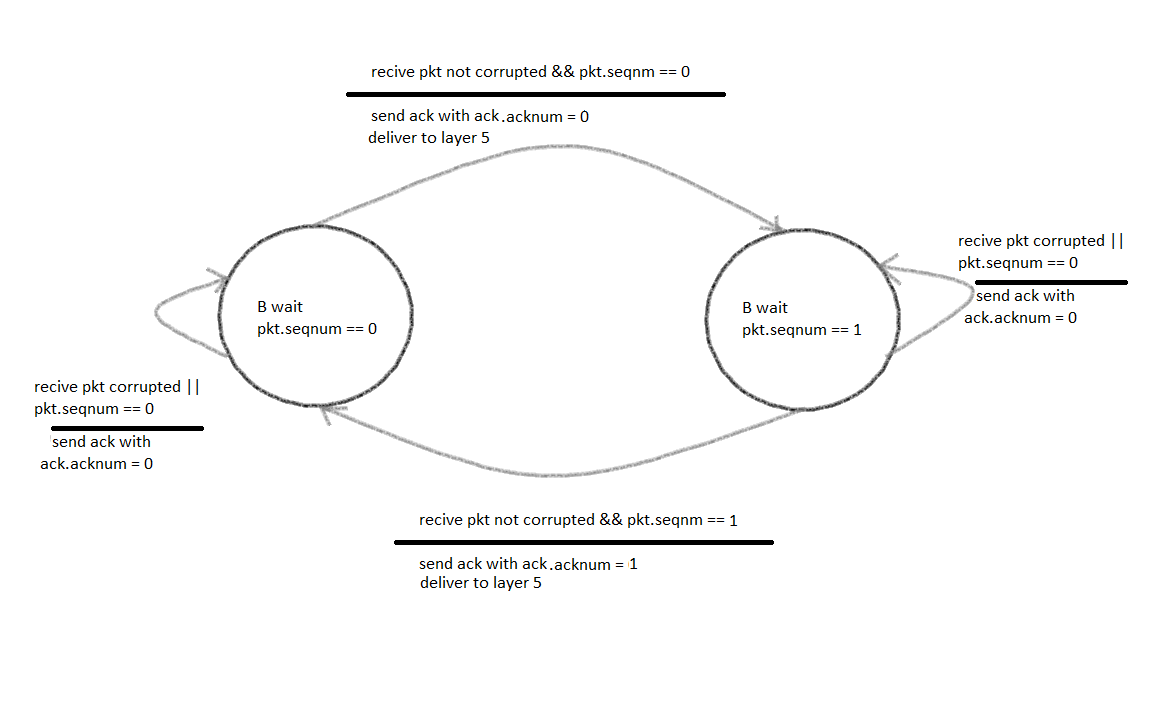
\includegraphics[scale = 0.30]{B.png}
\caption{Diagramma a stati entità B}
\end{figure}
 \newpage

\section{Test e Relativo output}
\subsection{Case 1}
\verbatiminput{okCase1OK.txt}
\subsection{Case 2}
\verbatiminput{okCase2OK.txt}

\end{document}